\begin{figure}[tbh]
	\centering
	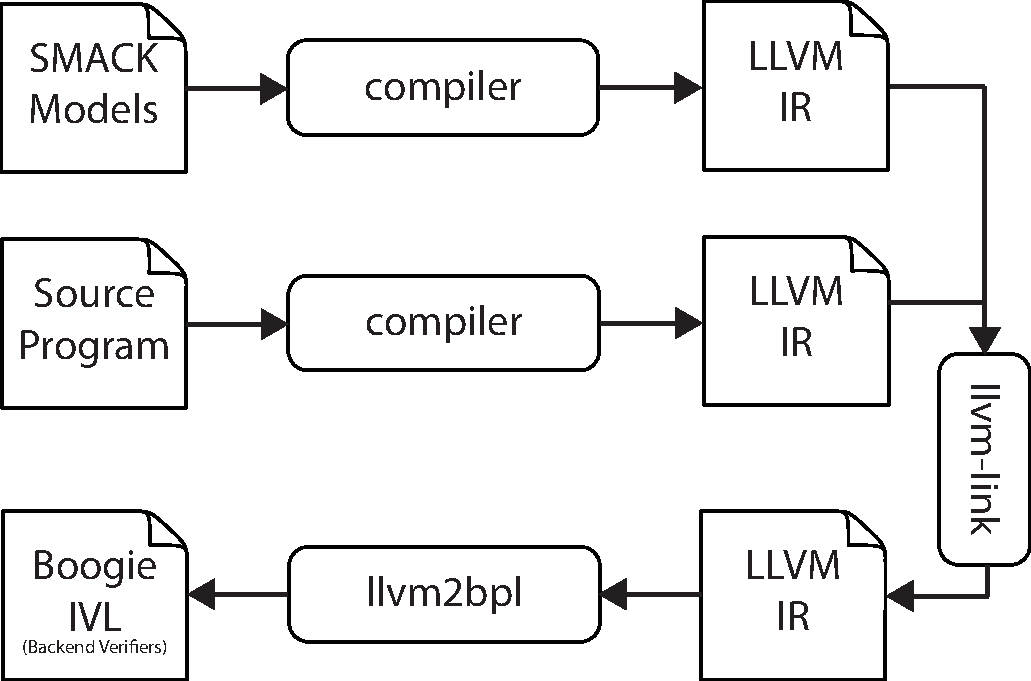
\includegraphics[width=\textwidth]{chap1/fig/SMACKIntro.pdf}
	\caption{Toolflow of SMACK.}
	\label{fig:vmcaitoolflow}
\end{figure}

%%%%%%%%%%%%%%%%%%%%%%%%%%%%%%%%%%%%%%%%%%%%%%%%%%%%%%%%%%%%%%%%%%%%%%%%%%%%%%%%%%%%%%%%%%

\begin{figure}[tbh]
%\begin{lstlisting}[language=Rust, label={lst:rustifc}, caption=Information flow control example in Rust., style=boxed, escapechar=`, float=tbh, captionpos=b, basicstyle=\small=]
\begin{lstlisting}[language=Rust, style=boxed, escapechar=`, captionpos=b, basicstyle=\small=]
fn check_label(x: SVec, l: Label) {
    verifier_assert!(x.l == l);
}

fn main() {
    let nd1: u64 = 5.verifier_nondet();
    let nd2: u64 = 5.verifier_nondet();
    let nd3: u64 = 6.verifier_nondet();

    // Ensure nd1 and nd3 have authorization greater than 4.
    // Ensure nd1 have at most the authorization of nd3.
    // Ensure nd2 have lower authorization than nd3.
    verifier_assume!(nd1 > 4 && nd3 > 4);
    verifier_assume!(nd1 <= nd3);
    verifier_assume!(nd2 < nd3);

    let mut s: SecVec = SecVec::new();
    let lsecret: SVec = svec![1,2,3 => nd1];
    let hsecret: SVec = svec![4,5,6 => nd3];

    // Add lsecret with nd1 authority.
    s.push(lsecret, nd1);`\label{line:lowauthadd}`
    // Update secret to hsecret with nd3 authority.
    s.update(0, hsecret, nd3);`\label{line:hiauthadd}`

    // Reading secrets with low authority
    match s.get(0, nd2) {`\label{line:lowauthacc}`
        None    => {},
        Some(sec) => {
            // Unreachable
            verifier_assert!(false);
            let label1 = sec;
            check_label(label1, nd2);
        }
    }

    // Reading secrets with high authority
    match s.get(0, nd3) {`\label{line:hiauthacc}`
        None      => {},
        Some(sec) => {
            let label2 = sec;
            // Check passes
            check_label(label2, nd3);
        }
    }
}
\end{lstlisting}
\caption{Information flow control example in Rust.}
\label{lst:rustifc}
\end{figure}

%%%%%%%%%%%%%%%%%%%%%%%%%%%%%%%%%%%%%%%%%%%%%%%%%%%%%%%%%%%%%%%%%%%%%%%%%%%%%%%%%%%%%%%%%%

\begin{figure}[tbh]
\begin{minipage}{.33\textwidth}
%\begin{lstlisting}[language=Rust, caption={Implementation of the factorial function in Rust.}, style=boxed, escapechar=`, captionpos=b, float=tbh, label=lst:factrs]
\begin{lstlisting}[language=Rust, style=boxed, escapechar=`]
fn fact(n: u32)
  -> u32
{
  let mut res = 1;
  for i in 1..=n
  {
    res *= i;
  }
  return res;
}
\end{lstlisting}
\end{minipage}
%
\begin{minipage}{.33\textwidth}
%\begin{lstlisting}[language=C, caption={Implementation of the factorial function in Swift.}, style=boxed, escapechar=`, captionpos=b, float=tbh,label=lst:factswift]
\begin{lstlisting}[language=C, style=boxed, escapechar=`]
func fact(n:UInt32)
  -> UInt32
{
  var result = 1
  for i in 1...n
  {
    result *= i
  }
  return result
}
\end{lstlisting}
\end{minipage}
%
\begin{minipage}{.33\textwidth}
%\begin{lstlisting}[language=C, caption={Implementation of the factorial function in C.}, style=boxed, escapechar=`, captionpos=b, float=tbh,label=lst:factc]
\begin{lstlisting}[language=C, style=boxed, escapechar=`]
uint32_t
fact(uint32_t n)
{
  uint32_t res = 1;
  for (uint32_t i = 1;
       i <= n; ++i) {
    res *= i;
  }
  return res;
}
\end{lstlisting}
\end{minipage}
\caption{Implementations of the factorial function in Rust (left), Swift (center) and C (right).}
\label{fig:factrsc}
\end{figure}

%%%%%%%%%%%%%%%%%%%%%%%%%%%%%%%%%%%%%%%%%%%%%%%%%%%%%%%%%%%%%%%%%%%%%%%%%%%%%%%%%%%%%%%%%%

\begin{figure}[tbh]
\begin{minipage}{.5\textwidth}
%\begin{lstlisting}[language=C, label={lst:muslacosfintro}, caption=Source of acosf.c from \texttt{musl} libm, style=boxed, escapechar=`, basicstyle=\small, float=tbh, captionpos=b]
\begin{lstlisting}[language=C, style=boxed, escapechar=`, basicstyle=\small]
float acosf(float x) {
  float z,w,s,c,df;

  uint32_t hx,ix;
  GET_FLOAT(hx, x);
  ix = hx & 0x7fffffff;
  /* |x| >= 1 or nan */
  if (ix >= 0x3f800000) {
    if (ix == 0x3f800000) {
      if (hx >> 31)
        return 2*pio2_hi +
               0x1p-120f;

      return 0;
    }
    return 0/(x-x);
  }
  /* |x| < 0.5 */
  if (ix < 0x3f000000) {
    /*|x|<2**-26*/
    if (ix<=0x32800000)
      return pio2_hi + 0x1p-120f;

    return pio2_hi - 
           (x-(pio2_lo-x*R(x*x)));
  }
  /* x < -0.5 */
  if (hx >> 31) {
    z = (1+x)*0.5f;
    s = sqrtf(z);
    w = R(z)*s-pio2_lo;
    return 2*(pio2_hi - (s+w));
  }
  /* x > 0.5 */
  z = (1-x)*0.5f;
  s = sqrtf(z);
  GET_FLOAT(hx,s);
  SET_FLOAT(df,hx&0xfffff000);

  c = (z-df*df)/(s+df);
  w = R(z)*s+c;
  return 2*(df+w);
}
\end{lstlisting}
\end{minipage}
%
\begin{minipage}{.5\textwidth}
%\begin{lstlisting}[language=Rust, label={lst:rustacosfintro}, caption=Source of acosf.rs from Rust libm, style=boxed, escapechar=`, basicstyle=\small, captionpos=b, float=tbh]
\begin{lstlisting}[language=Rust, style=boxed, escapechar=`, basicstyle=\small]
fn acosf(x: f32) -> f32 {
  let x1p_120 =
    f32::from_bits(0x03800000);
  let z:f32;let w:f32;let s:f32;
  let mut hx = x.to_bits();
  let ix = hx & 0x7fffffff;
  /* |x| >= 1 or nan */
  if ix >= 0x3f800000 {
    if ix == 0x3f800000 {
      if (hx >> 31) != 0 {
        return 2. * PIO2_HI +
               x1p_120;
      }
      return 0.;
    }
    return 0. / (x - x);
  }
  /* |x| < 0.5 */
  if ix < 0x3f000000 {
    if ix <= 0x32800000 {
      /* |x| < 2**-26 */
      return PIO2_HI + x1p_120;
    }
    return PIO2_HI -
           (x-(PIO2_LO-x*r(x*x)));
  }
  /* x < -0.5 */
  if (hx >> 31) != 0 {
    z = (1. + x) * 0.5;
    s = sqrtf(z);
    w = r(z) * s - PIO2_LO;
    return 2.*(PIO2_HI - (s + w));
  }
  /* x > 0.5 */
  z = (1. - x) * 0.5;
  s = sqrtf(z);
  hx = s.to_bits();
  let df =
    f32::from_bits(hx&0xfffff000);
  let c = (z-df*df)/(s+df);
  w = r(z) * s + c;
  2. * (df + w)
}
\end{lstlisting}
\end{minipage}
\caption{Implementations of the \texttt{acosf} function in \texttt{musl} libm (left) and Rust libm (right).}
\label{fig:acosfintro}
\end{figure}
